% !TeX spellcheck = en_US
\chapter{System description}
The project is a collection of three individually developed systems, who as a whole makes it possible to test and control the AU2.

\section{AU2}
The MCU(Motor control unit) can be seen in figure

\begin{figure}[h!]
\centering
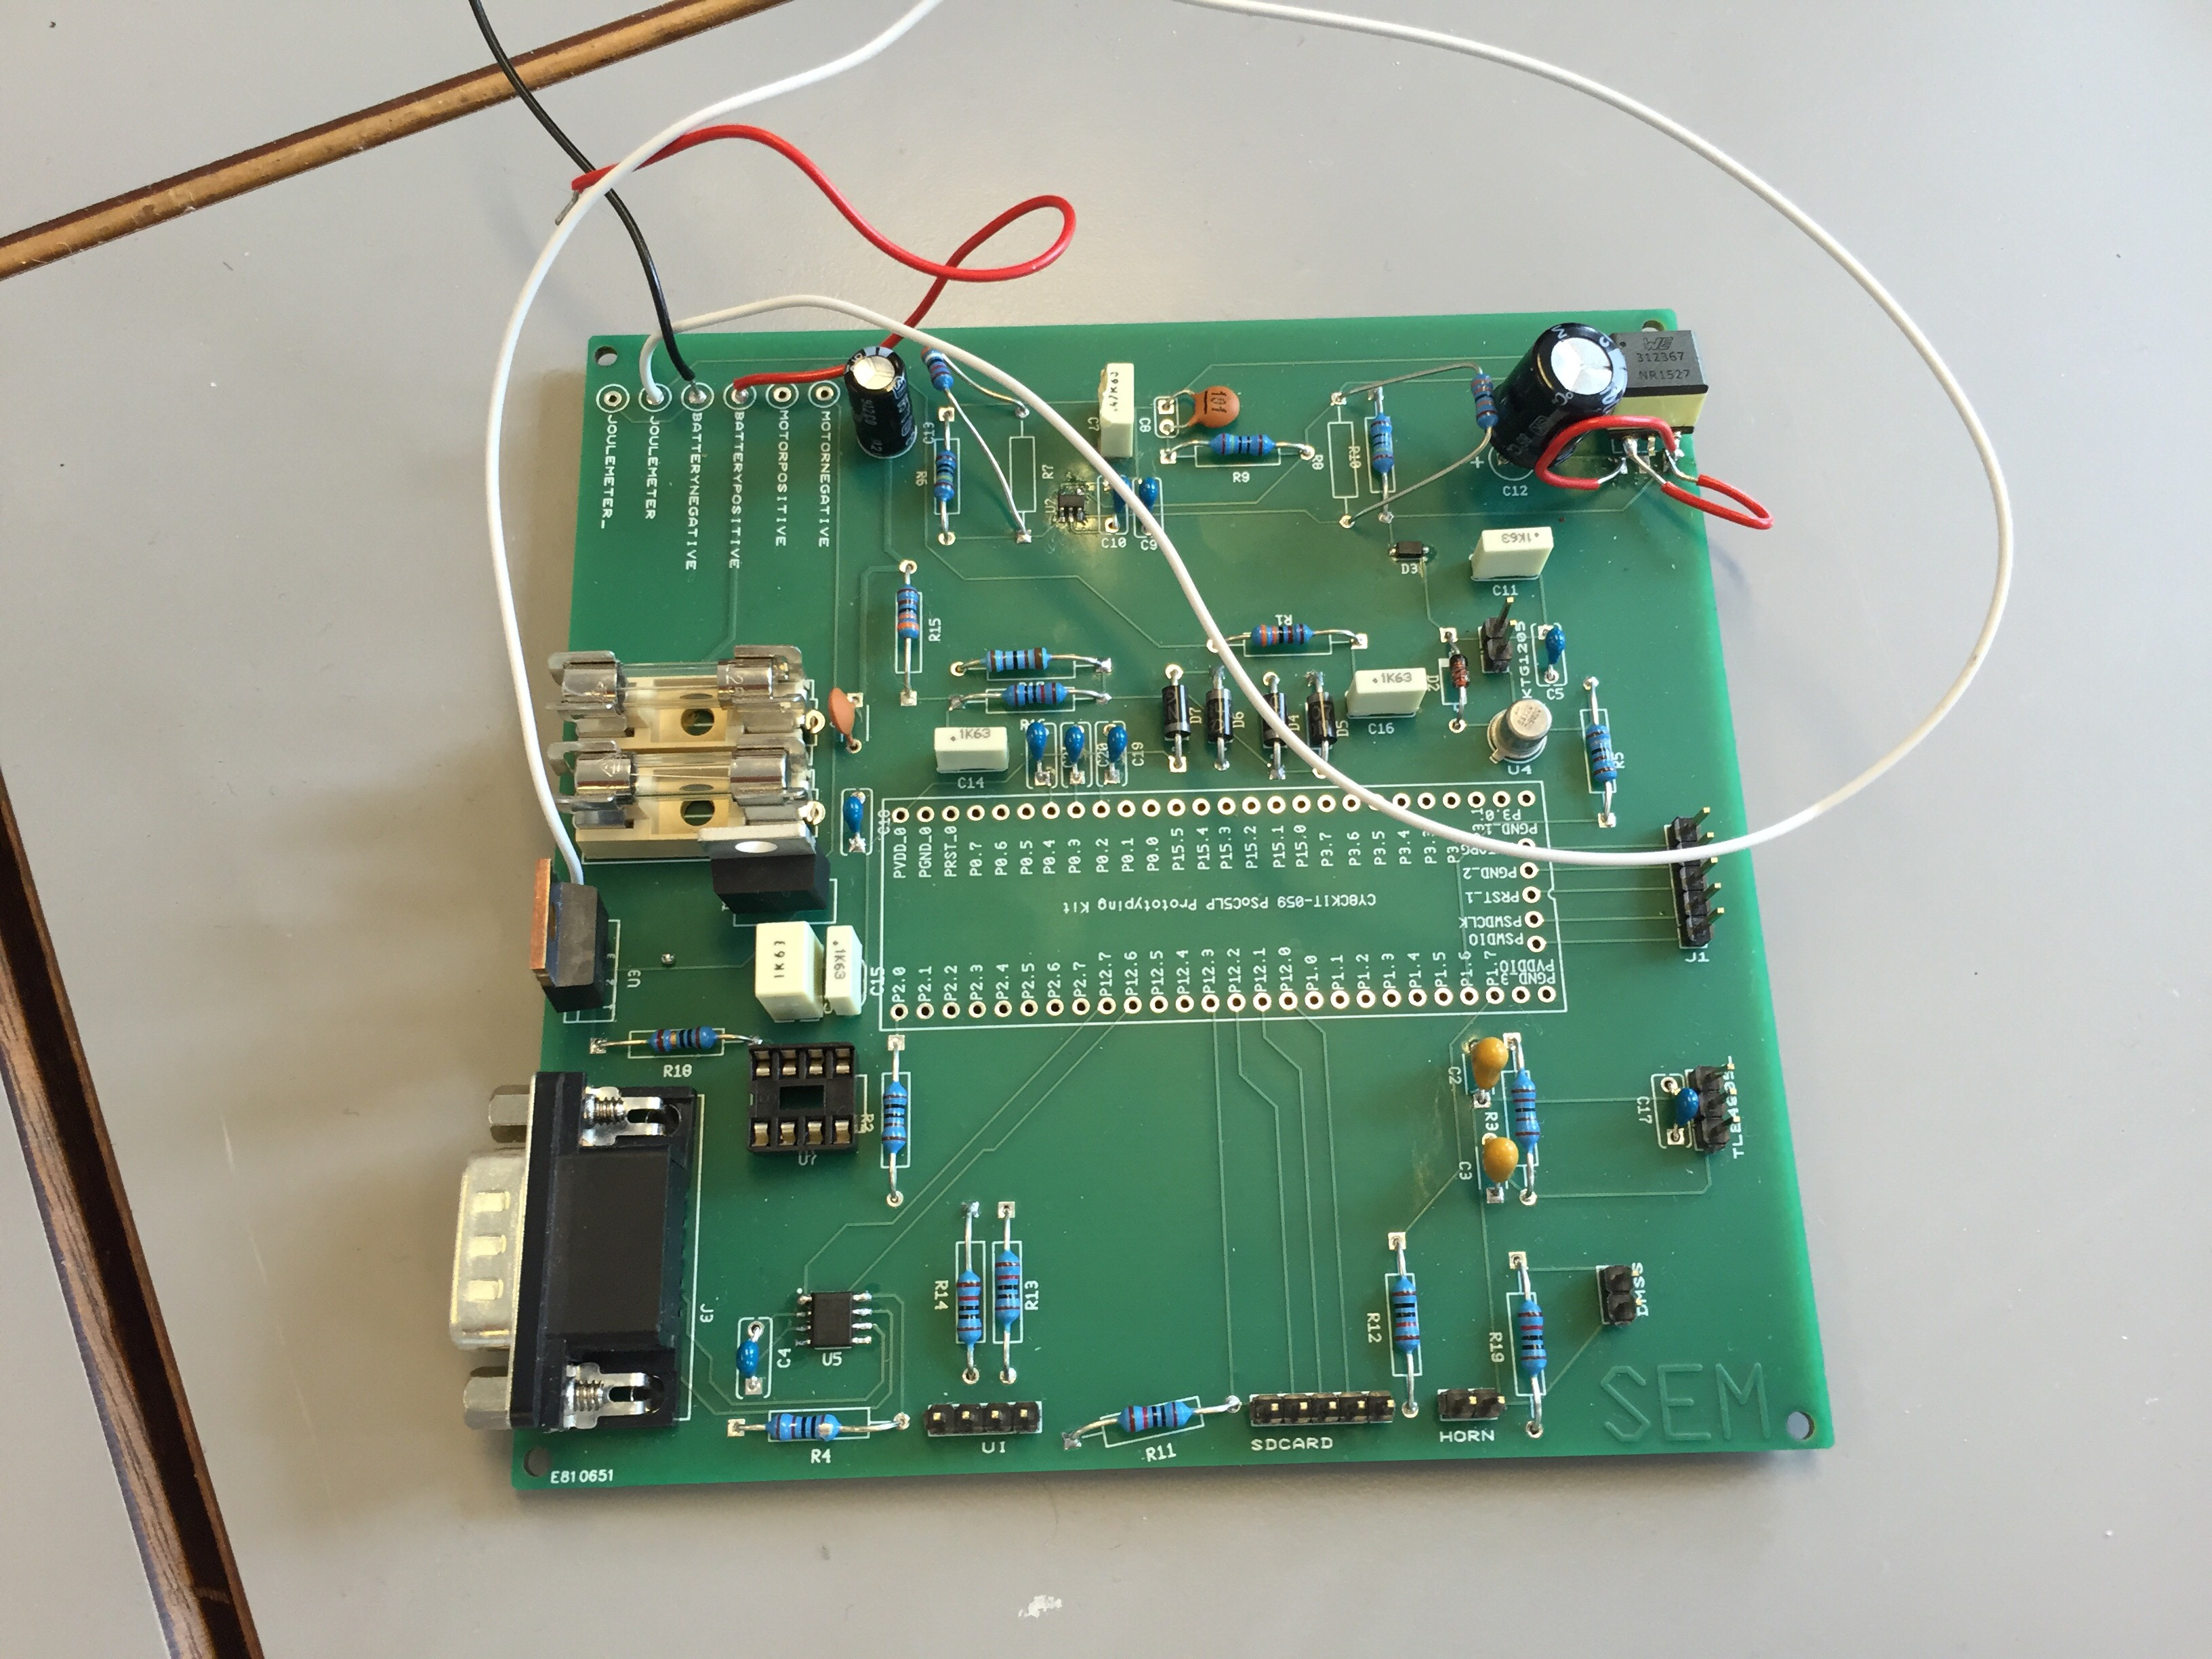
\includegraphics[width=0.7\linewidth]{SubPages/Images/SD_MCS}
\caption{}
\label{fig:SD_MCS}
\end{figure}

The BMS(Battery manage system)

\begin{figure}[h!]
\centering
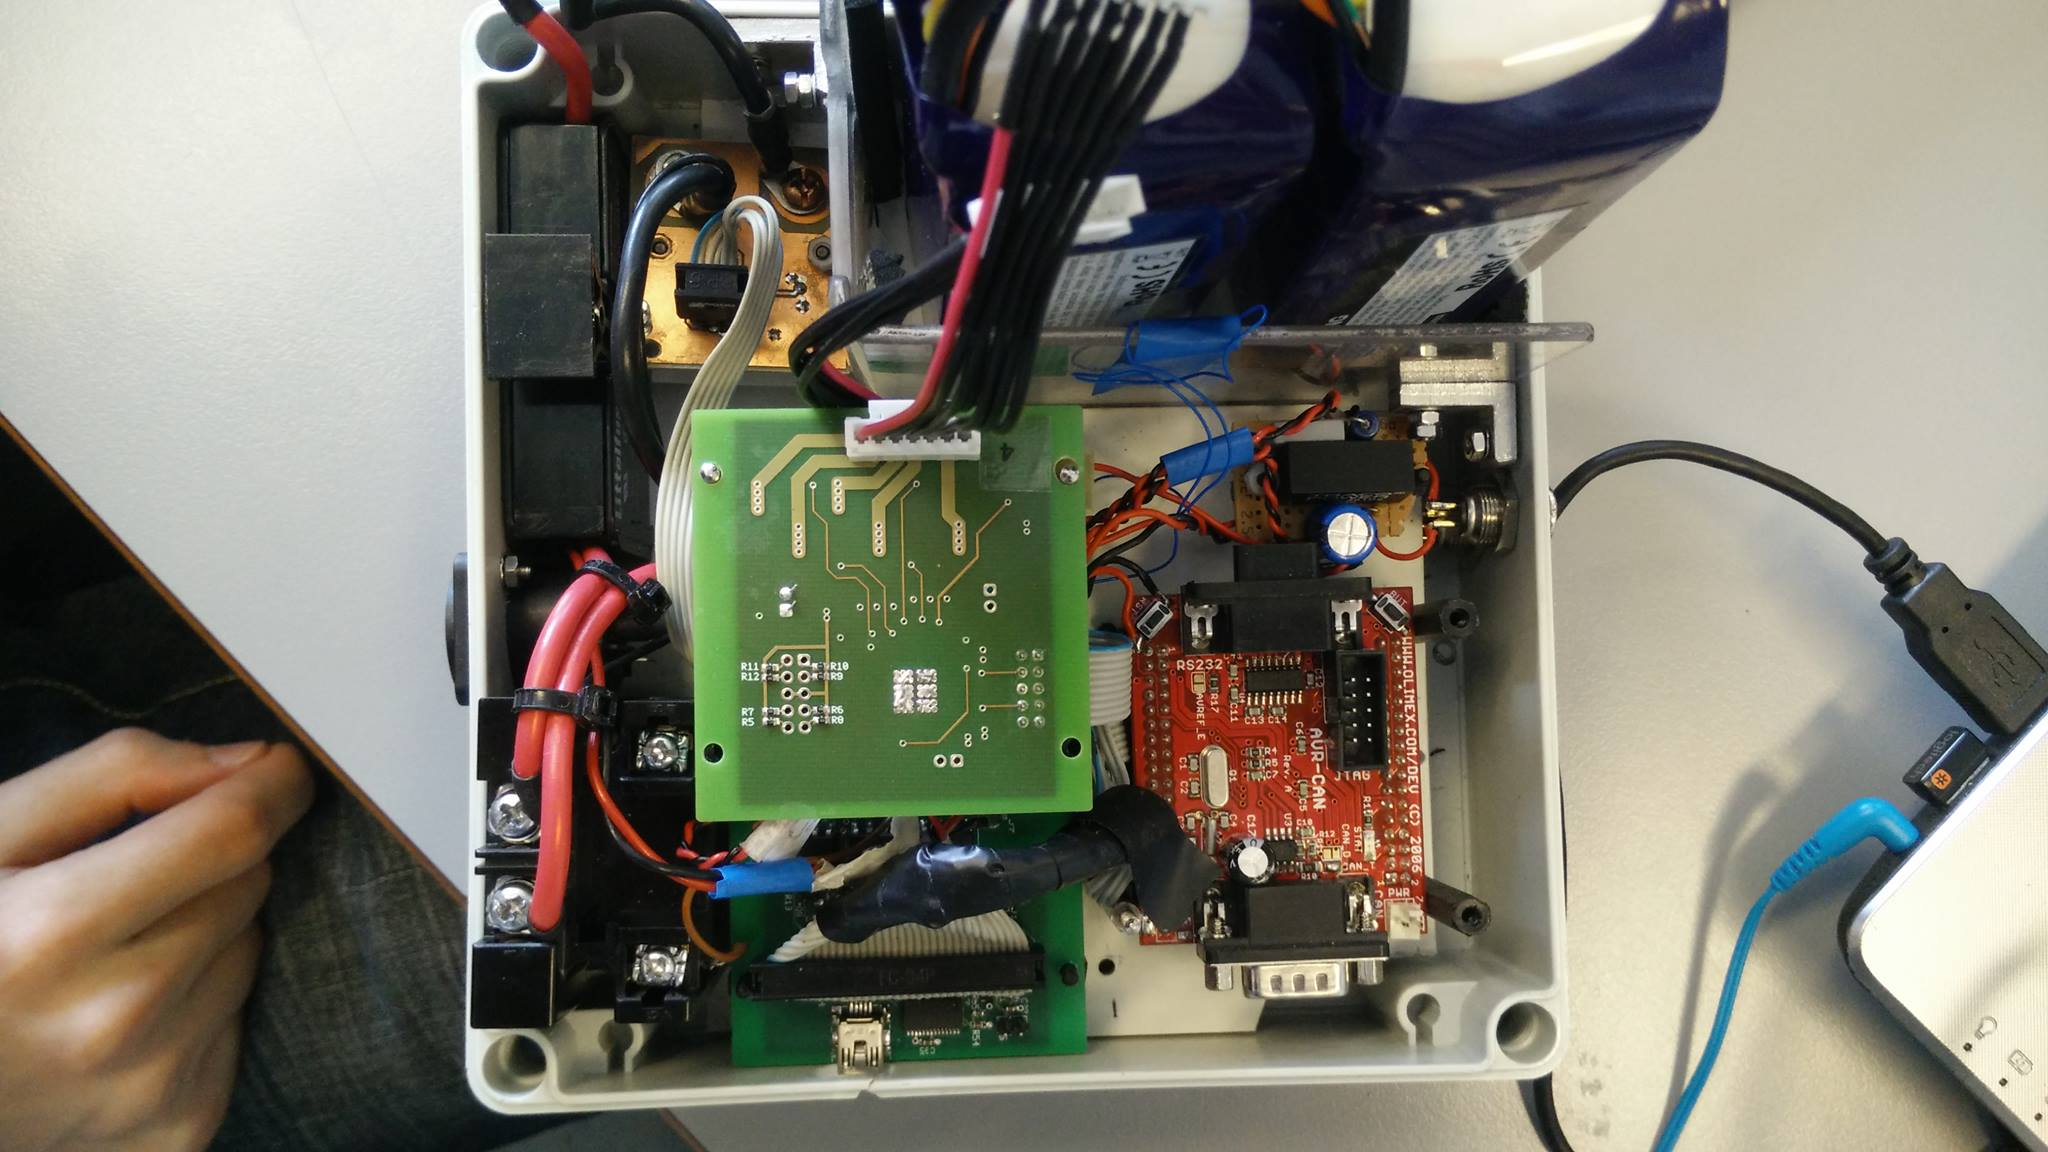
\includegraphics[width=0.7\linewidth]{SubPages/Images/SD_BMS}
\caption{}
\label{fig:SD_BMS}
\end{figure}

\section{Rolling Road}
The Controller-box containing the PCB can be seen in figure \vref{fig:SD_RR}.

\begin{figure}[h!]
\centering
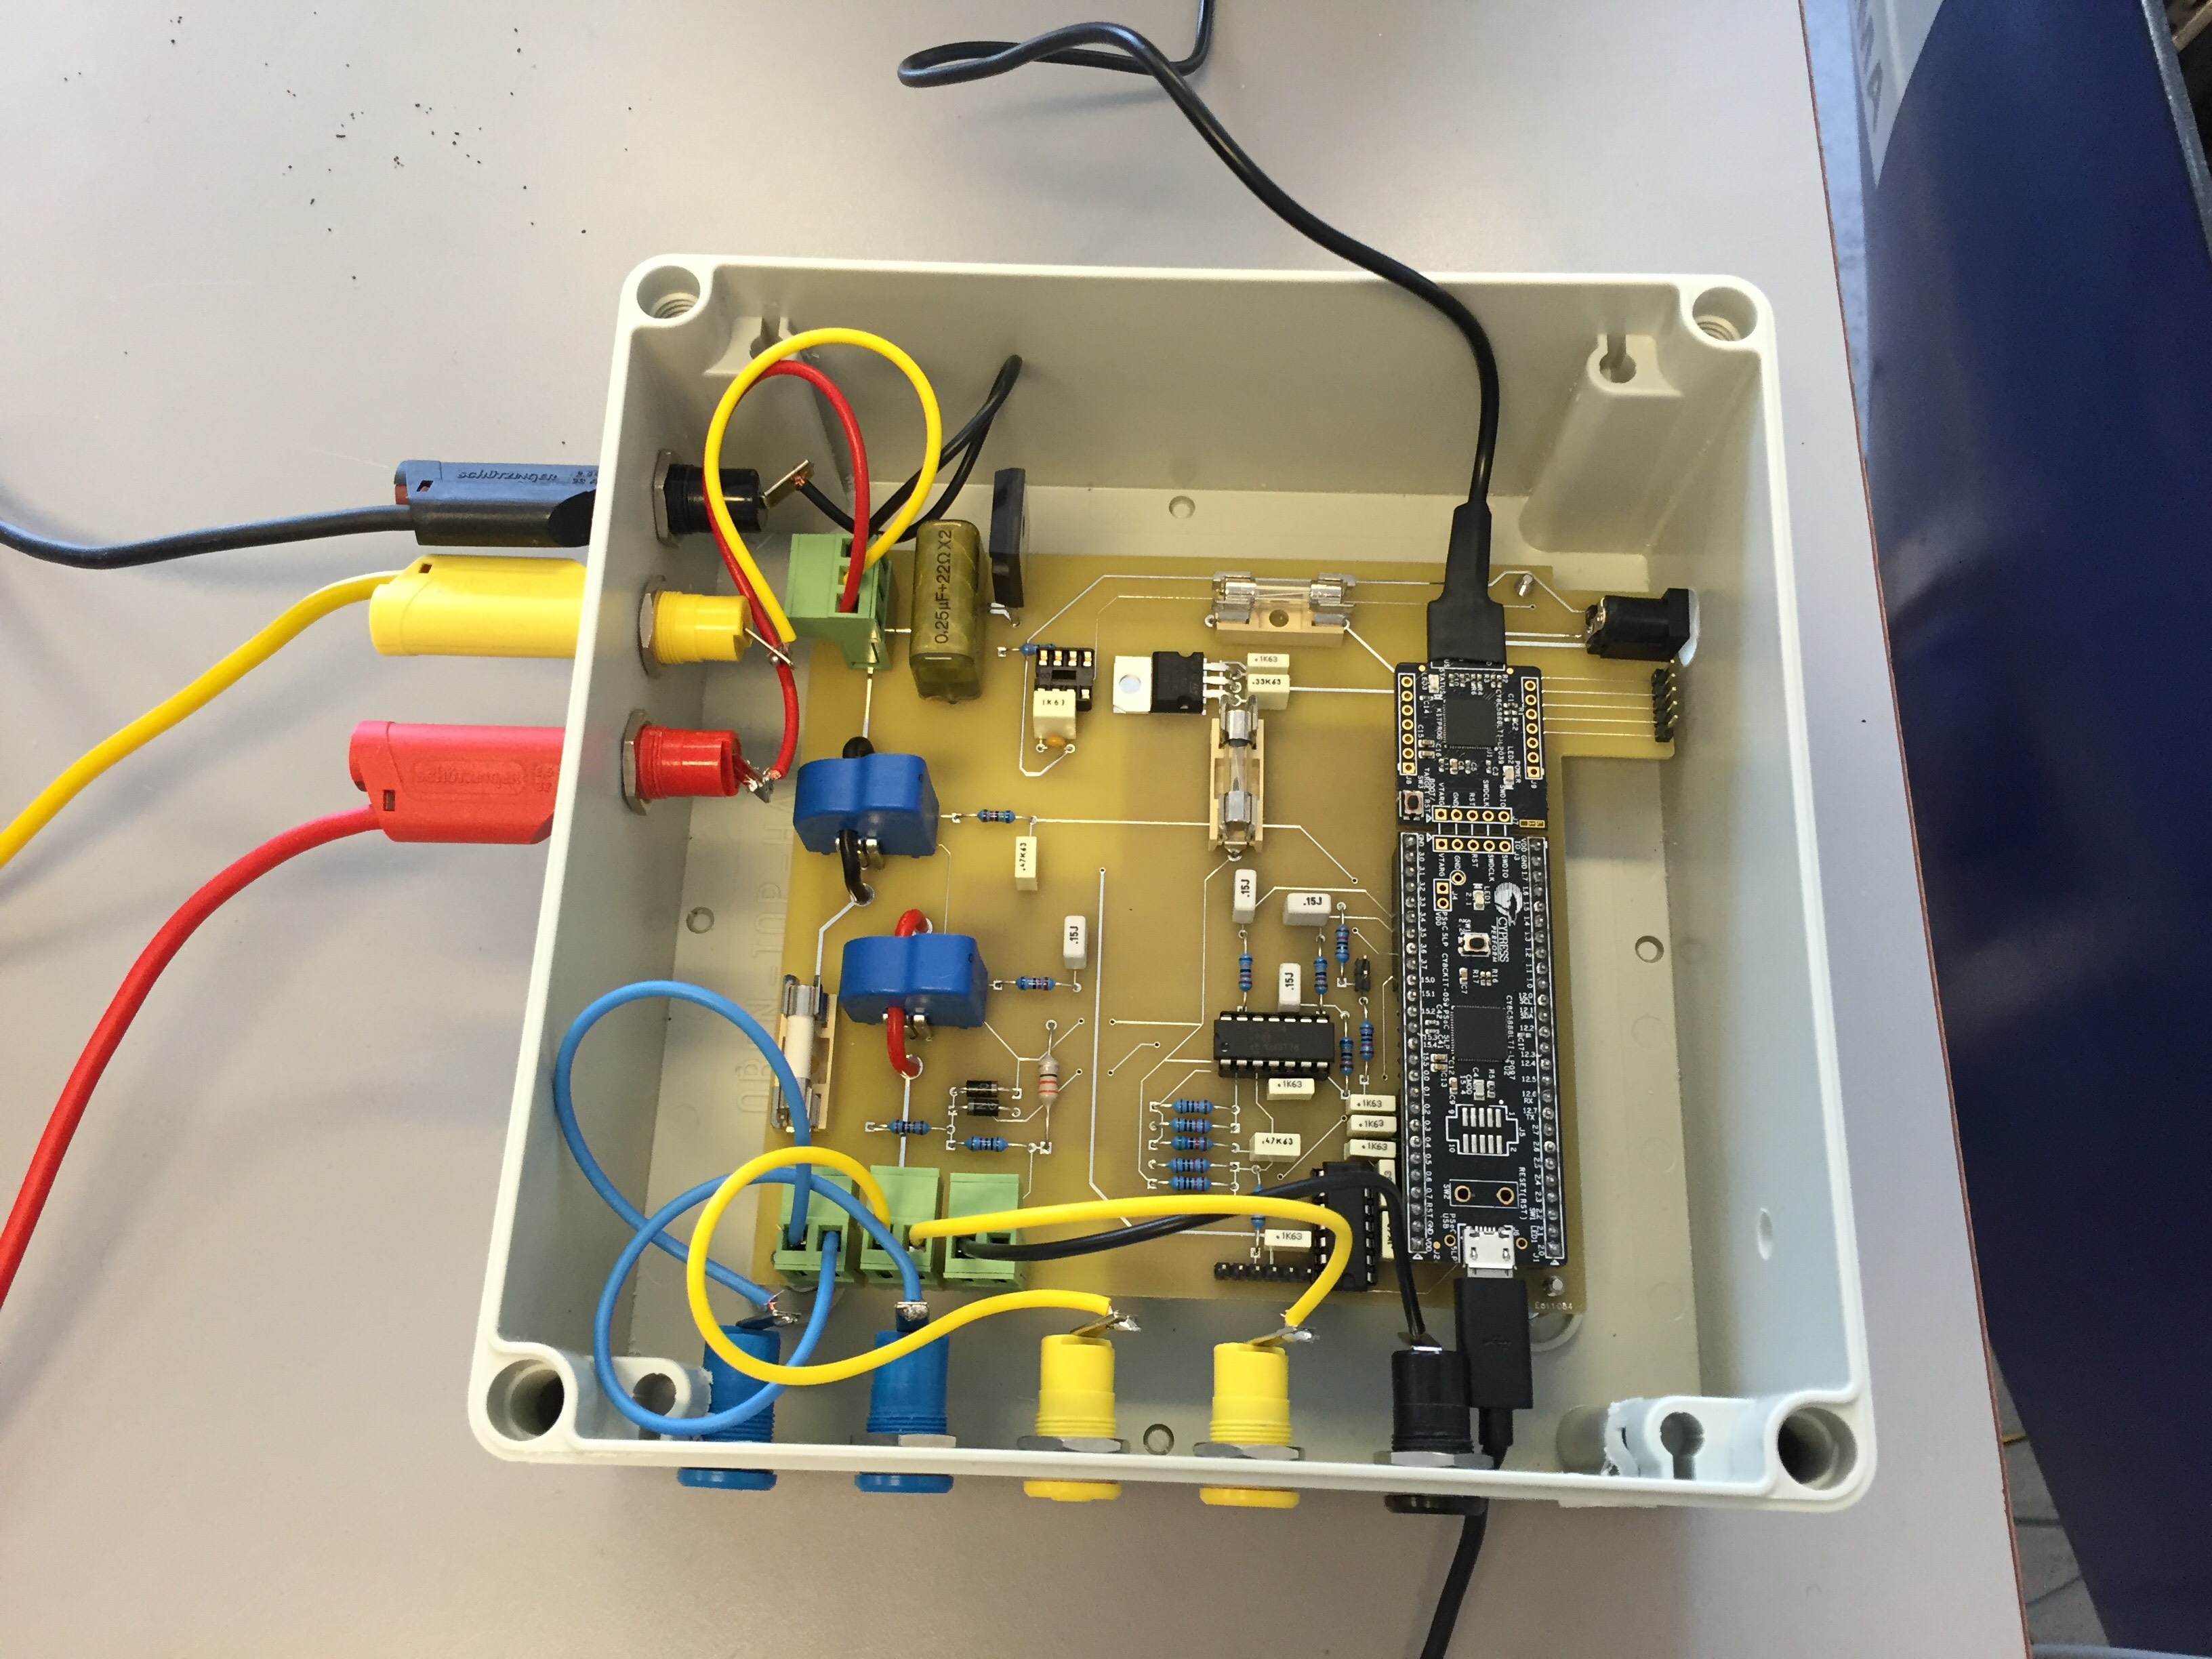
\includegraphics[width=0.7\linewidth]{SubPages/Images/SD_RR}
\caption{Controller}
\label{fig:SD_RR}
\end{figure}


The Physical stand containing the generator and torque sensor can be seen in figure \vref{fig:SS_RR_Roal}.

\begin{figure}[h!]
\centering
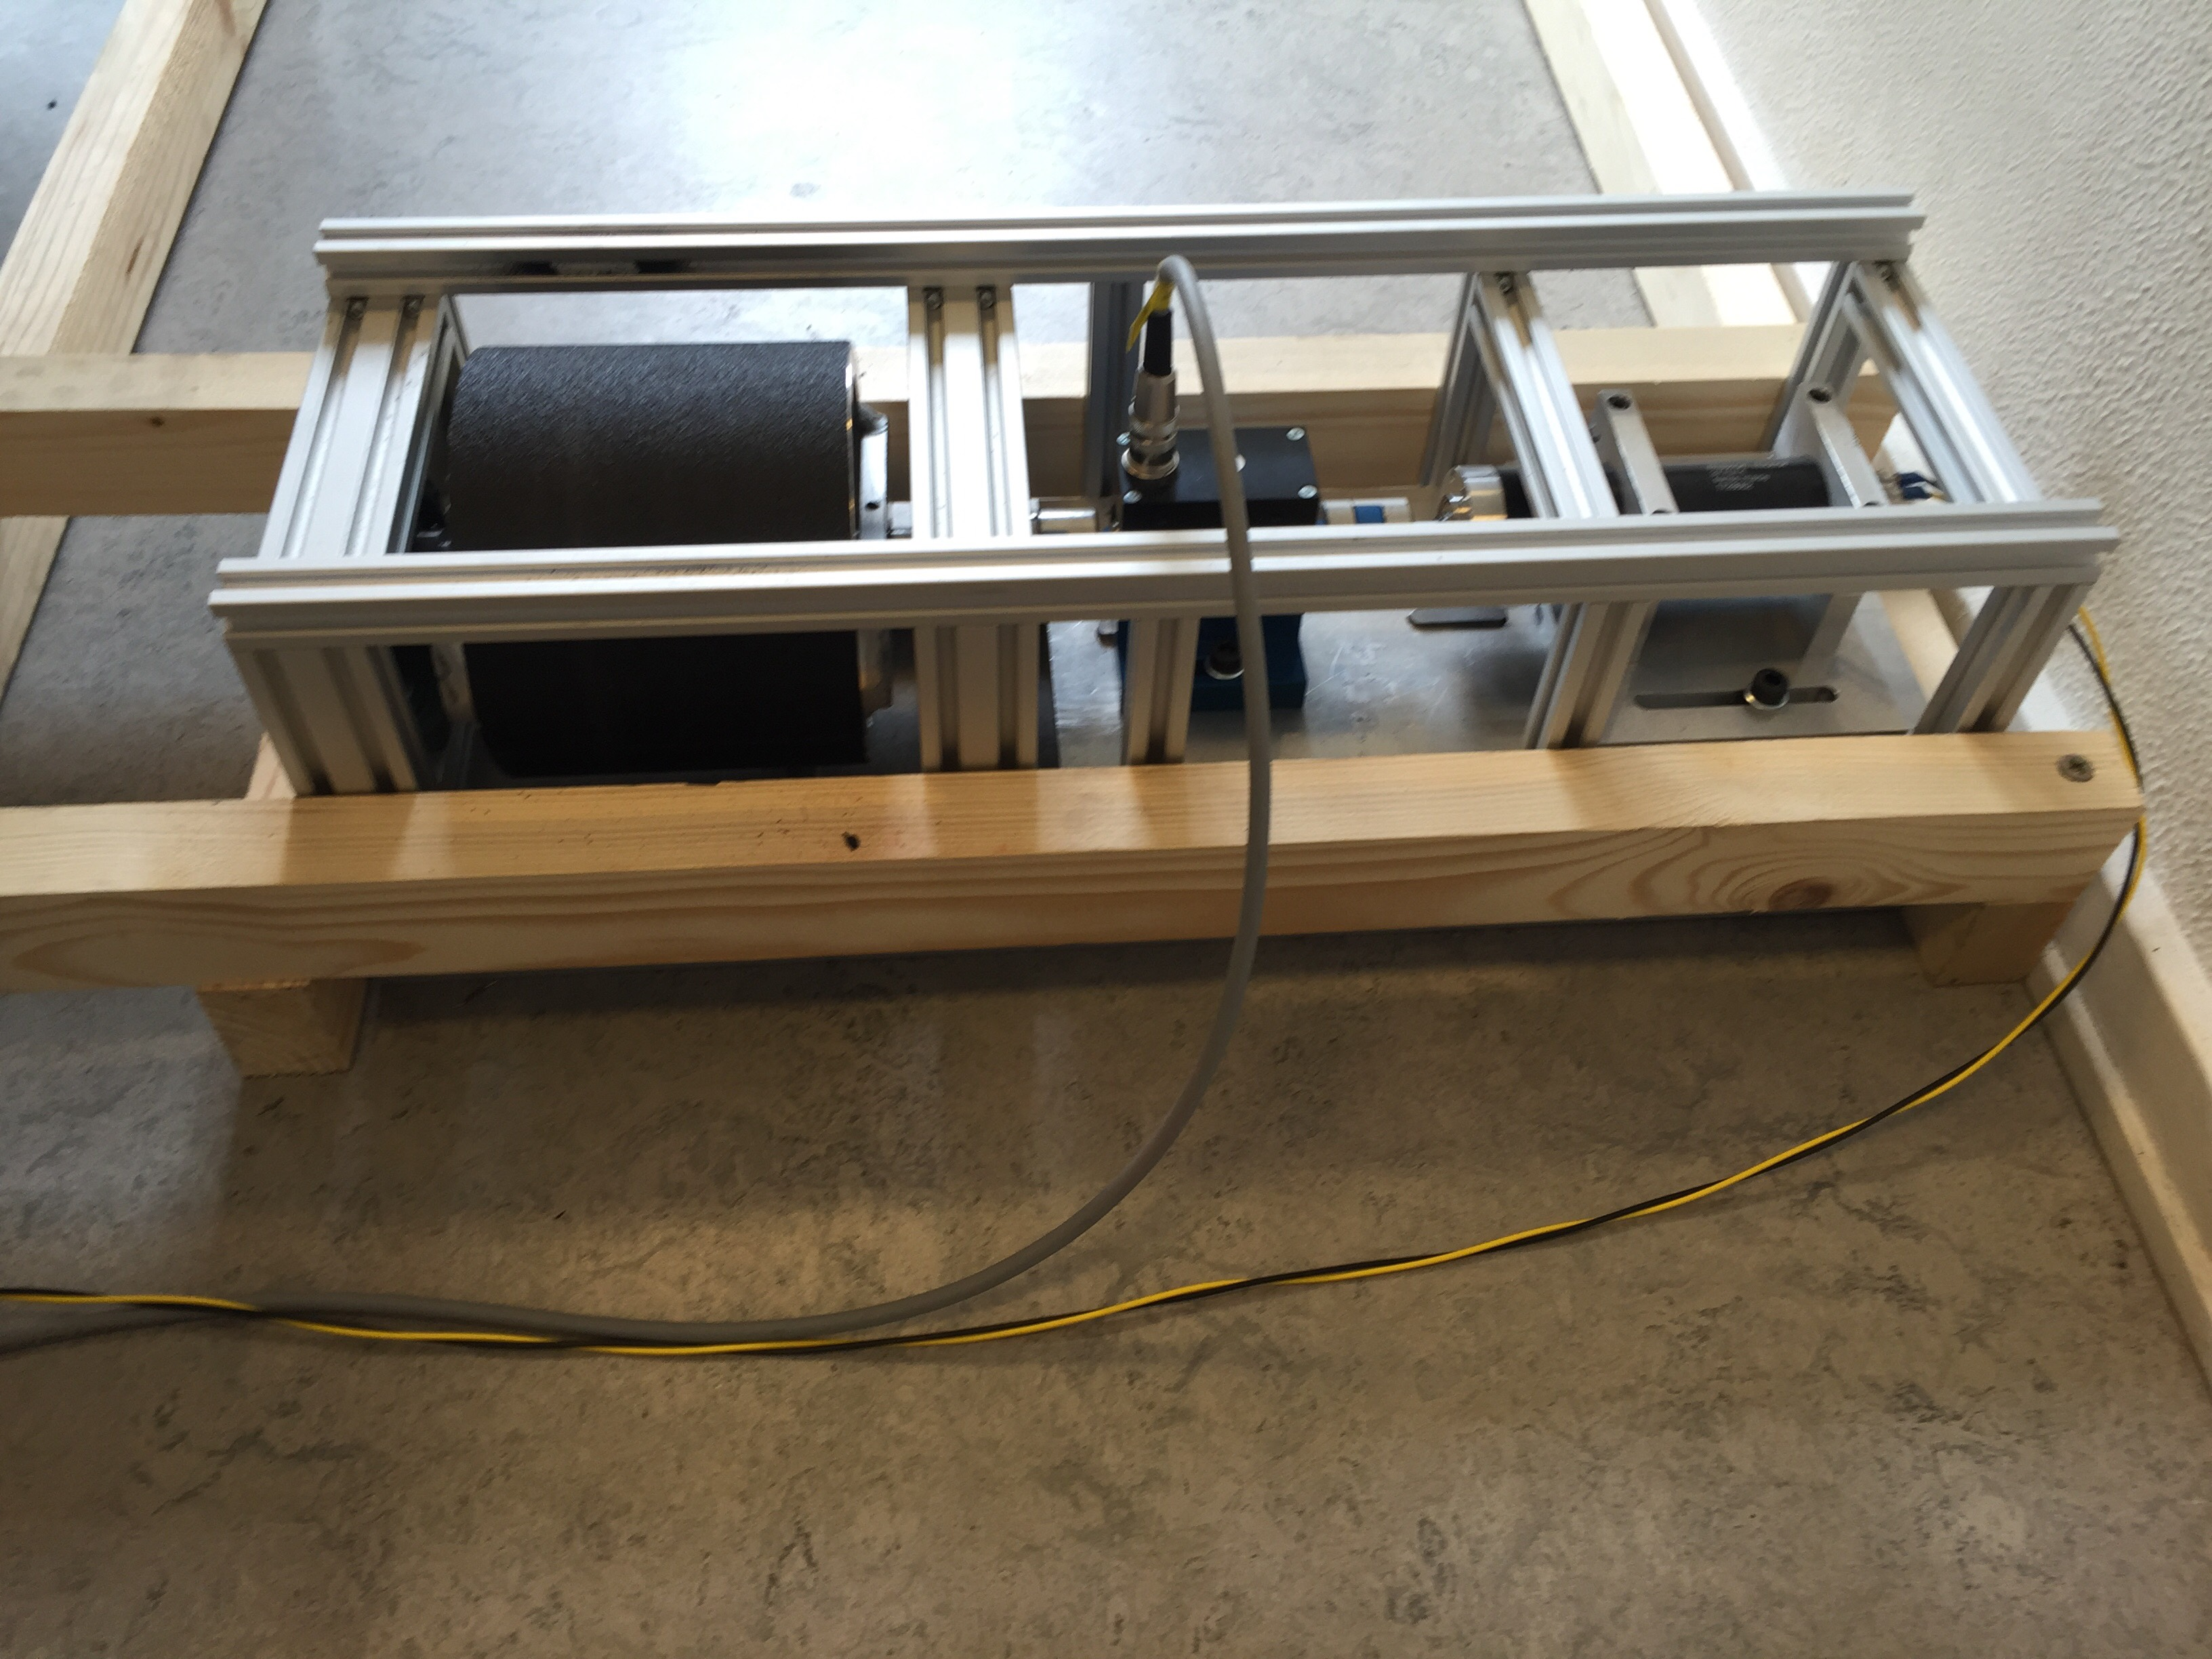
\includegraphics[width=0.7\linewidth]{SubPages/Images/SS_RR_Roal}
\caption{Rolling Road}
\label{fig:SS_RR_Roal}
\end{figure}


The Load-plate containing the super capacitor and the power resistors:

\begin{figure}[h!]
\centering
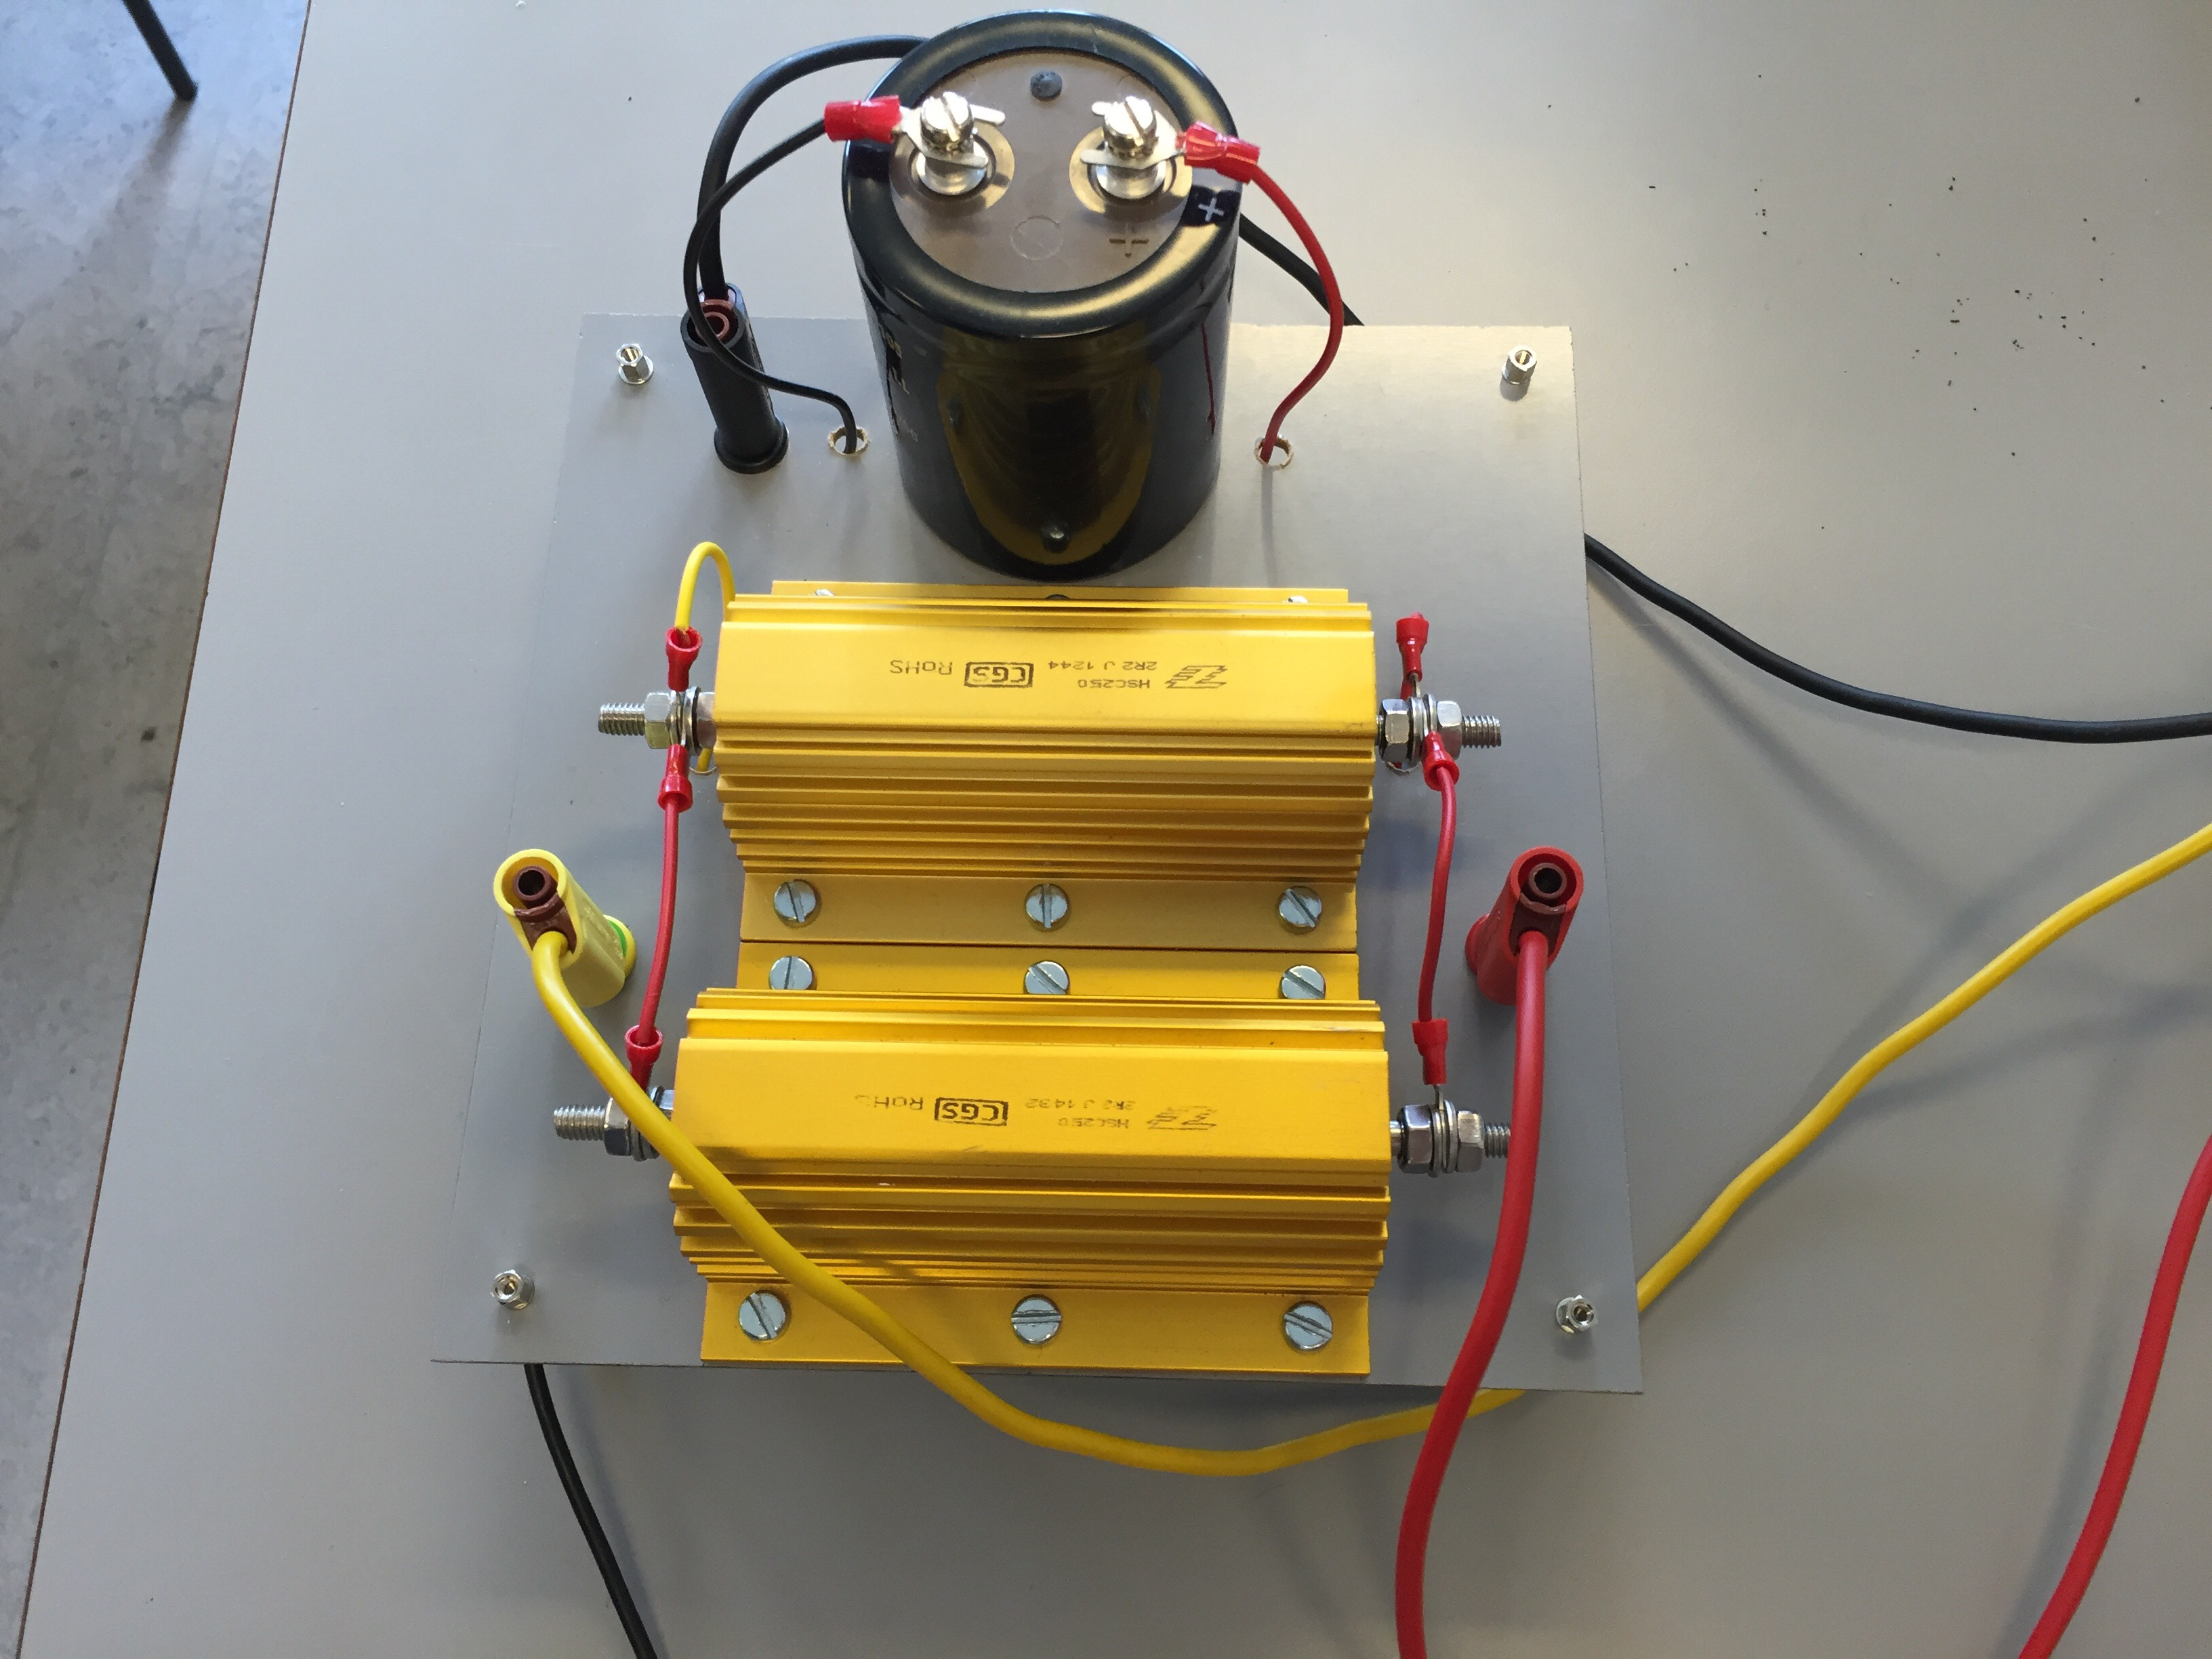
\includegraphics[width=0.7\linewidth]{SubPages/Images/SD_RR_Load}
\caption{Load}
\label{fig:SD_RR_Load}
\end{figure}


\section{Rolling Road GUI}
The best software EU

\begin{figure}[h!]
\centering
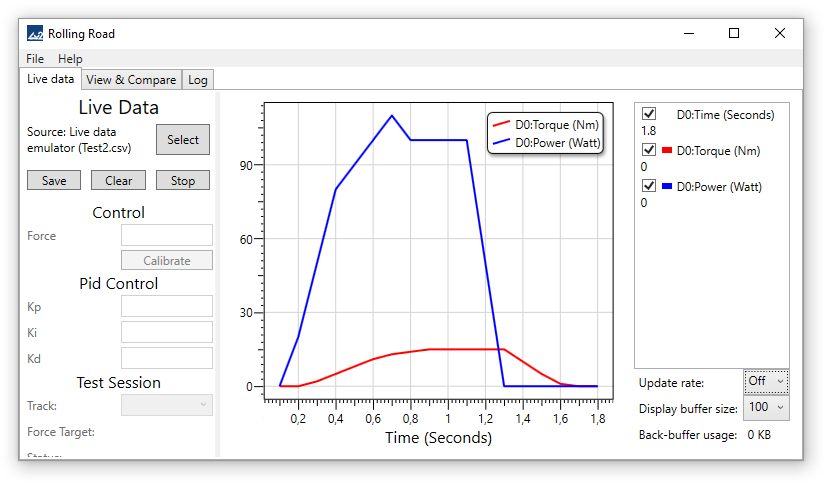
\includegraphics[width=0.9\linewidth]{SubPages/Images/SD_GUI}
\caption{}
\label{fig:SD_GUI}
\end{figure}
